Spatial commonsense, \cite{liu2022things}, is knowledge about the spatial positions of objects and the relationships between them 
(for examples, relationships regarding the sizes of objects in an image or the distances between objects in an image, etc).
In spatial commonsense reasoning, there are two main approaches in research: object scale — the relative size differences between objects 
in an environment, and spatial relationship — the spatial connections between objects or humans within a space. 

With object scale problems, the research \cite{aroca2021prost}, published in 2021, introduced a dataset with 18,736 multiple-choice questions (fill-in-the-blanks) 
using 14 different templates related to physical reasoning abilities, including 10 basic concepts such as: direction, mass, height, circumference, stackable, rollable, graspable, breakable, slideable, and bounceable
he questions were created with 14 different templates, each template represented in the following three formats: direction templates — questions related to the direction and position of objects in the sentence; 
attributes templates — related to features such as mass, height, etc.; and affordance templates — related to the capabilities of objects: stackable, rollable, etc. 
Based on the dataset they previously developed, the authors evaluated three models: Decoder model — OpenAI’s GPT-1, Encoder model — BERT, and Encoder-decoder Models — T5 using zero-shot prompting. 
The results showed that these models were influenced by the order of answer options and questions with reversed meanings, and increasing the number of parameters and pretraining data did not significantly improve the results.
However, the results were evaluated and analyzed long before the advent of new large language models with enhanced capabilities, such as GPT-4 and Llama. Therefore, the conclusions are only relevant at that time, 
but the research also introduced a method for evaluating the reliability of spatial reasoning abilities in LLMs.

To analyze the spatial relationship reasoning abilities of LLMs, the study \cite{hudson2019gqa} introduced the GQA (Generalized Question Answering) dataset to evaluate this problem. They utilized the structure of the Visual Genome scene graph
to generate 22 million diverse questions with corresponding functional programs. The goal of developing this dataset was to address the shortcomings of the earlier VGA dataset
GQA consists of 113K images and 22M questions, measuring the performance of models in spatial reasoning skill suchs as: object and
attribute recognition, transitive relation tracking, spatial reasoning, logical inference and comparisons. The image, questions and corresponding answers are represented as follows: each image is annotated with a dense Scene Graph — 
capturing information about the objects present in the image, their attributes, and the relationships between these objects.  Subsequently, each image is paired with a function that describes the reasoning steps needed to arrive at the answer.



The study \cite{liu2022things} introduces a benchmark for evaluating the reasoning abilities of LLMs in general and VLLMs in particular in spatial commonsense, and conducts experiments across various models. 
The benchmark combines the relative sizes of objects and their interactions with one another. Evaluation was carried out on two types of models: vision-language models — which combine images and language for reasoning, 
and image synthesis models — which generate images from descriptions or context. The authors found that image synthesis models performed significantly better at learning and reasoning about spatial relationships compared to the other models.


\begin{figure}
    \centering
    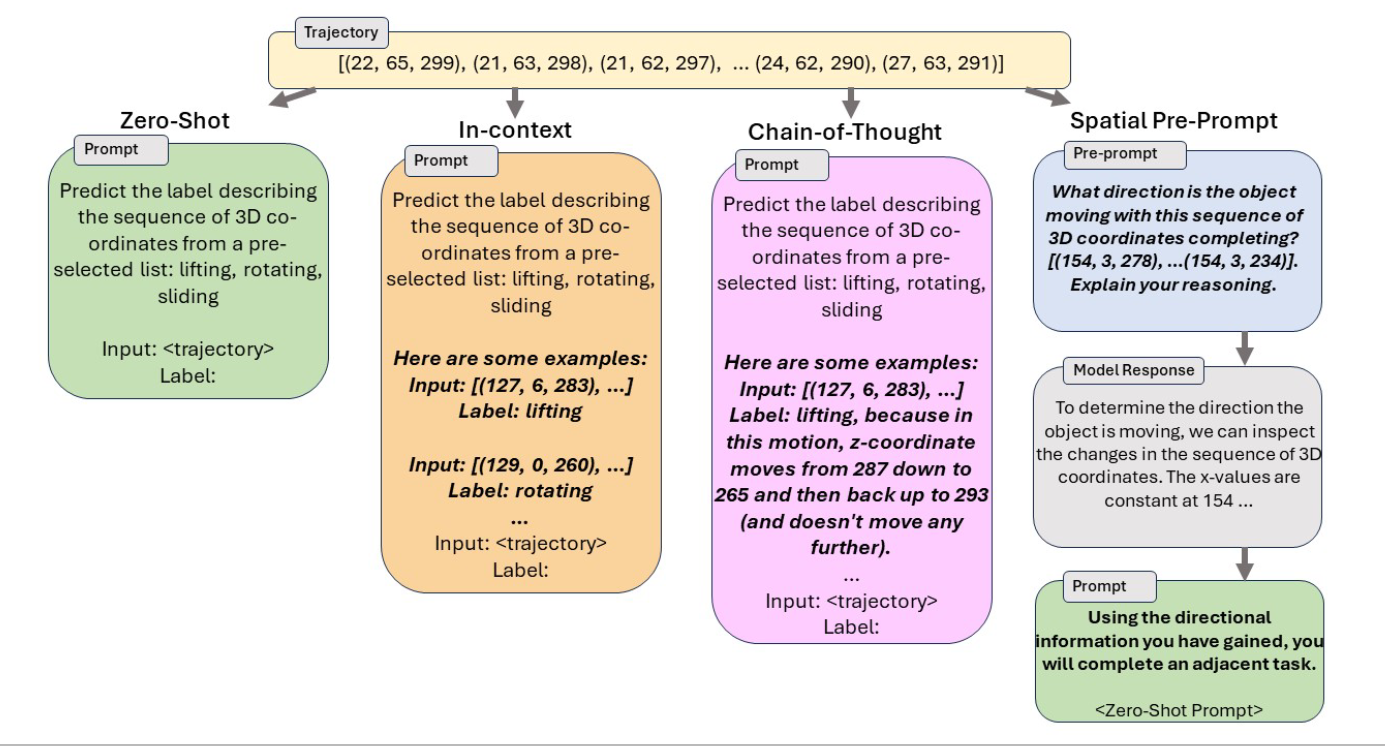
\includegraphics[width=0.9\textwidth]{Figs/SPP.png}
    \caption{Different Types of Prompting Mechanisms - Zero-shot, In-context Learning, Chain-ofThought and Spatial Prefix-Prompting.}
    \label{fig:spp}
\end{figure}

Another study \cite{sharma2023exploring} focused on improving the reasoning capabilities of LLMs like Llama, ChatGPT, etc., when processing 3D trajectory data of robots from the CALVIN dataset. The tasks involved include 2D directional and shaping labels. 
Unlike the datasets mentioned above, this dataset contains only the 3D coordinates of objects moving in space. Additionally, the researchers introduced a new method called prefix-based prompting, which improved the performance of LLMs by up to 33\% on the 3D trajectory dataset 
and by 10\% on the SpatialQA dataset using zero-shot prompting. The study found that while LLMs perform well on natural language reasoning tasks, they struggle with shape recognition and handling spatial relationships. Methods like in-context learning and chain-of-thought (CoT) prompting can enhance LLMs' reasoning capabilities; however, 
the authors’ Spatial Prefix-Prompting (SPP) method (\ref{fig:spp}) outperformed these approaches on most benchmarks. SPP works by using a set of simple, pre-prepared questions to encourage LLMs to answer and reason through straightforward problems first. The reasoning derived from these questions is then used to tackle more complex related questions
Not only does this method surpass CoT and few-shot learning in benchmarks, but it is also more efficient as it does not require explicit reasoning steps (as CoT does) and avoids bias introduced by provided examples (as in few-shot learning). 



